\chapter{Contaminaci\'on Atmosf\'erica}

\section{Fuentes de gases a la atmósfera}

En esta sección se verán las diferentes fuentes que interviene en la emisión de compuestos gaseosos que se encuentran en la atmósfera

\subsection{Biológicas}\index{fuentes!biologicas@biológicas}\label{subbio}
\begin{itemize}
\item Fotosíntesis de las plantas, responsables del oxígeno (\ce{O2}) de la atmósfera
\item  Respiración libera \ce{CO2} en el aire.
\item  Metano (\ce{CH4}), es liberado de materiales orgánicos, de la fermentación de vacas, termitas, humedales, cultivos de arroz y tundra.
\item  Terpenos  se evaporan de las hojas, al oxidarse producen partículas y en conjunto con el NOx produce ozono. 
\item Otros gases generados en la biosfera (\ce{CO} y \ce{N2O}) se relacionan con el control de ozono.
\item Quema de biomasa emite gases y partículas a la atmósfera. Las especies reactivas de la quema de biomasa inducen un incremento en la producción de ozono y especies del esmog.
\item  Transformaciones biológicas el \ce{N2} a \ce{NH3}, \ce{N2O} y \ce{NO}.
\item Regiones oceánicas de alta productividad biológica y contenido orgánico, zonas de surgencia, aguas costeras y las marismas costeras son la principal fuente de bisulfuro de carbono (\ce{CS2})  y sulfuro de carbonilo. (COS). El fitoplancton emite dimetilsulfato (\ce{CH3SCH3} DMS) y bisulfuro de dimetilo (\ce{CH3SSCH3}). La degradación microbiana de materia orgánica muerta libera ácido sulfhídrico (\ce{H2S}).
\item Fuentes importantes de cloruro de metilo (\ce{CH3Cl}), que es el halocarbono más abundante en el aire, incluyen la actividad biológica en el agua de mar, los mohos de la madera y la quema de biomasa. El cloruro de metilo es la principal fuente natural de cloro estratosférico.
\item El hidrógeno molecular se emite por la actividad microbiana en los océanos, quema de biomasa, la fermentación bacteriana de suelos y la fotólisis del formaldehído.
\item El uso por parte de los seres humanos de materiales biogénicos da lugar a emisiones de numerosos químicos tóxicos a la atmósfera.
\end{itemize}
\begin{example} Un modelo simple de intercambio de COS entre la capa superficial del océano, donde se genera, y las regiones inferiores de océano se pueden basar en las siguientes consideraciones. a) el COS en las capa superficial del océano está en equilibrio con el COS de la atmósfera y no hay sumidero atmosférico neto, b) La concentración de COS en la superficie del océano, C(0), es constante a $1.0\times10^{-11}$\kilogrampercubicmetre. c) Debajo de la superficie del océano el COS se destruye químicamente con  un coeficiente de tasa de primer orden $k=5.0\times10^{-6}$\per\second. d)  Debajo de la misma capa superficial, la destrucción química de COS se equilibra con el transporte descendente de remolinos con un coeficiente de difusión de 0.0050 \metre\per\square\second. e) El océano es infinitamente profundo y uniforme en la horizontal. Utilice estos supuestos para determinar:
\begin{enumerate}
\item ¿A qué profundidad la concentración de COS en el océano es igual a C(0)/2?
 \item  La densidad de la columna de COS en el océano.
 \item La vida media de una molécula de COS en el océano.
 \end{enumerate}
 
\textbf{Solución}. Dado que el océano es uniforme en la horizontal, sólo necesitamos considerar la transferencia en la dirección vertical (z) (es decir, podemos usar un modelo unidimensional (1D)). Considere una pequeña porción de océano a una distancia z debajo de la superficie del océano que tiene una unidad de área de sección transversal y espesor $dz$ (figura \ref{COS_fig}). Sea $F(z)$ el flujo de COS hacia la parte superior de esta losa y $F(z + dz)$ el flujo que sale de la base de la losa. El flujo neto de COS hacia la losa es
 
 \begin{figure}[hbtp]
\begin{center}
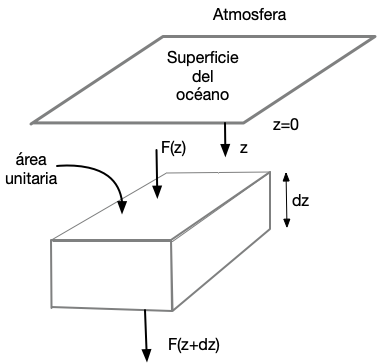
\includegraphics[width=0.50\textwidth]{COS_model.png}
\caption{Diagrama del ejercicio}
\label{COS_fig}
\end{center}
\end{figure}

\begin{equation}
\Delta F=F(z)-F(z+\mathrm{d}z)=F(z)-\left[ F(z)+\frac{\mathrm{d}F(z)}{\mathrm{d}z}\mathrm{d}z \right]=-\mathrm{d}F(z)
\end{equation}
Como el volumen de la losa es $1\cdot \mathrm{d}z$ 
\begin{equation}
\textrm{el flujo neto de COS en una unidad de volumen de la losa} =-\frac{\mathrm{d}F(z)}{\mathrm{d}z}
\label{flux_COS}
\end{equation}
Si $D$ coeficiente de difusión en remolino,
\begin{equation}
F(z)=-D\frac{\mathrm{d}C(z)}{\mathrm{d}z}
\label{dif_COS}
\end{equation}
donde $C(z)$ es la concentración de COS a la distancia $z$ debajo de la superficie del océano, y el signo negativo surge porque la difusión ocurre en la dirección opuesta a la del aumento de la concentración. En el presente caso, la concentración de COS es mayor en la superficie del océano y disminuye hacia abajo; por lo tanto, el flujo de COS es descendente en el océano. De las ecuaciones. (\ref{flux_COS}) y (\ref{dif_COS})
\begin{equation}
\textrm{el flujo neto de COS en una unidad de volumen de la losa} =D\frac{\mathrm{d}^2C(z)}{\mathrm{d}z^2}
\label{flux2_COS}
\end{equation}
\noindent Si $k$ es el coeficiente de tasa de primer orden para la destrucción química de COS en aguas marinas 

\begin{equation}
\textrm{tasa de destrucción de COS en una unidad de volumen de la losa} =kC(z)
\label{des_COS}
\end{equation}
\noindent En condiciones de estado estacionario, de las ecuaciones (\ref{flux2_COS}) y  (\ref{des_COS})
\begin{equation}
\frac{\mathrm{d}C(z)}{\mathrm{d}t}=D\frac{\mathrm{d}^2C(z)}{\mathrm{d}z^2}-kC(z)=0
\label{cc_COS}
\end{equation}
La solución de la ecuación~\ref{cc_COS} es
\begin{equation}
C(z)=C(0)\exp(-z/H)
\label{c_cos}
\end{equation}
\noindent donde H (una altura de escala) está dada por
\begin{equation}
H=\left( \frac{D}{k}\right)^{1/2} =  \left( \frac{0.0050}{5.0\times10^{-6}}\right)=32 \metre
\label{H_COS}
\end{equation}

Ahora se pueden responder las tres preguntas:

\begin{enumerate}
\item Cuando $C(z)=C(0)/2$, tenemos de las ecuaciones (\ref{c_cos}) y  (\ref{H_COS}) 
\begin{equation*}
\frac{1}{2}=\exp\left(-\frac{z}{H} \right)=\exp\left( -\frac{z}{32}\right)
\end{equation*}
Por lo tanto, z = 22m
\item La densidad de la columna de COS en el océano es la masa total de COS en una columna de unidad de área de sección transversal que se extiende desde la superficie hasta el fondo del océano. Por lo tanto
\begin{eqnarray*}
\textrm{Densidad de columna de COS} &=& \int_{z=0}^\infty C(z)\,\mathrm{d}z \\
       &=&  \int_{z=0}^\infty C(0)\exp\left(-\frac{z}{H}\right)\,\mathrm{d}z  \\
       &=& C(0)H \\
       &=& (1.0\times10^{-11})\times 32 \\
       &=& 3.2\times10^{-10}\kilogrampersquaremetre 
\end{eqnarray*}
%
\item De la ecuación de tiempo de vida de un compuesto $\tau=\frac{M}{F}$
donde $M$ es la cantidad de sustancia química en, digamos, la columna de sección transversal unitaria que consideramos anteriormente y $F$ es la salida (tasa de eliminación más tasa de destrucción) de la sustancia química de la columna. Por lo tanto, la vida media de una molécula de COS en el océano viene dada por:
\begin{eqnarray*}
\tau & = & \frac{C(0)H}{k\int_0^\infty C(z)\,\mathrm{d}z } \\
& =& \frac{C(0)H}{kC(0)H}  \\ 
& =& \frac{1}{k}  \\ 
&=& \frac{1}{5.0\times10^{-6} \per\second}\\
&=& 2.3  \textrm{ dias} 
\end{eqnarray*}
\end{enumerate}
\end{example}
\subsection{Tierra sólida}\index{fuentes!tierra@tierra sólida}
Los volcanes son la fuente geoquímica más importante de gases traza en al atmósfera. Aunque son muy localizados y muy variables, cuando las emisiones volcánicas son lanzadas a la estratosfera (o superior), pueden dispersarse rápidamente por todo el mundo y tener largos tiempos de residencia (1 a 2 año). El polvo fino  llega a dar varias vueltas alrededor de la Tierra. Los aerosoles producidos a partir de los gases pueden permanecer en la estratosfera durante varios años. Esto, a su vez, da lugar a un enfriamiento medio global en la superficie de $\sim0.4\degreecelsius$ en el año siguiente a la erupción; este enfriamiento llega a desaparecer después de $\sim$3 años a medida que disminuye el polvo en la atmósfera. Además de cenizas y partículas de polvo, los volcanes emiten \ce{H2O}, \ce{CO2}, \ce{SO2}, \ce{H2S}, COS, \ce{CS2}, HCl, HF, HBr, \ce{CH4}, \ce{CH3Cl}, \ce{H2}, CO y varios metales pesados volátiles (p. ej., Hg). Las rocas son una fuente de  cantidades pequeñas de ciertos gases y son las principales fuentes de los gases He, Ar y Rn en la atmósfera. El helio se produce principalmente del decaimiento radiactivo del uranio-238 y torio-232- No se acumula en la atmósfera debido a que es tan ligero que escapa de la exosfera\index{exosfera}. El argón se ha acumulado durante eones debido a la desintegración radiactiva del potasio-40 de rocas.

Las rocas carbonatadas, como la piedra caliza, que se presenta principalmente como calcita (es decir, \ce{CaCO3}), contienen 100,000 veces más carbono que la atmósfera, pero la mayor parte está secuestrada. Sin embargo, las rocas carbonatadas y los sedimentos marinos participan en un ciclo de período largo con el \ce{CO2} atmosférico como se muestra a continuación. La erosión de la calcita por el \ce{CO2} disuelto en la lluvia y en aguas dulces (ríos y lagos) se puede representar por

\begin{footnotesize}
\begin{eqnarray}
\ce{CO2}(g) + \ce{H2O} &\rightleftarrows& \ce{CO2}(ac) + \ce{H2O}(l)  \label{eq_co2h2o}\\
\ce{2H2O}(l) +   \ce{CO2}(ac)&\rightleftarrows&   \ce{H3O^+}(ac) +  \ce{HCO3^-}(ac) \label{eq_co2}\\
\ce{CaCO3}(s) +   \ce{H3O^+}(ac) +  \ce{HCO3^-}(ac) &\rightleftarrows& \ce{Ca^{2+}}(ac) + \ce{2HCO3^-}(aq) + \ce{H2O}(l)\label{eq_caco3}\\\hline
\textrm{Neto:       }   \ce{CaCO3}(s) +\ce{CO2}(g) + \ce{H2O}(l)  &\rightleftarrows&\ce{Ca^{2+}}(ac) + \ce{2HCO3^-}(aq)  \label{eq_cca}
\end{eqnarray}
\end{footnotesize}

La reacción (\ref{eq_co2h2o}) representa el equilibrio entre el \ce{CO2} en el aire y en los ríos y lagos de agua dulce. En la reacción (\ref{eq_co2}), el \ce{CO2} recibe un \ce{OH^-}  del \ce{H2O} para formar el ácido muy débil (es decir, poco ionizado) \ce{HCO3^-} (el ion bicarbonato), y en la reacción (\ref{eq_caco3}) el \ce{H3O+} remueve \ce{CO3^{2-}} del \ce{CaCO3} para formar otro ion bicarbonato\index{bicarbonato}. La reacción directa de (\ref{eq_caco3}) representa la erosión de la calcita por el \ce{CO2}  disuelto en aguas dulces.

Los productos de la \gloss[word]{meteorizacion} en el lado derecho de la Reacción (\ref{eq_cca}) eventualmente ingresan a los océanos, donde se precipitan para formar nuevos sedimentos (lo contrario de la Reacción (\ref{eq_cca})). A través del levantamiento de las regiones de la plataforma continental, la subducción de sedimentos marinos hacia el manto superior y la corteza inferior de la Tierra y las erupciones volcánicas, estos productos eventualmente regresan a los sedimentos continentales, completando así este ciclo geoquímico. Los tiempos de residencia del \ce{Ca^{2+}}(aq) y del \ce{HCO3^-}(aq) en los océanos son $\sim 8\times 10^5$ y $\sim7.5 \times 10^4$ años, respectivamente.

\begin{example}
Cuando el \ce{CO2} se disuelve en agua pura ¿que reacciones se producen?

\textbf{Respuesta:}

\begin{footnotesize}
\begin{eqnarray}
\ce{CO2}(g) + \ce{H2O} &\rightleftarrows& \ce{H2CO3}(ac) \\
\ce{H2CO3}(ac) + \ce{H2O}(l) &\rightleftarrows&  \ce{HCO3^-}(ac) + \ce{H3O^+}(ac) \\
 \ce{HCO3^-}(ac) + \ce{H2O}(l) &\rightleftarrows&  \ce{CO3^{-2}}(ac) + \ce{H3O^+}(ac) \\ \hline
 \textrm{Neto:         } \ce{CO2}(g) + 3\ce{H2O} &\rightleftarrows& \ce{CO3^{-2}}(ac) +2 \ce{H3O^+}(ac) 
 \end{eqnarray}
\end{footnotesize}
\end{example}

\subsection{Oc\'eanos}\index{fuentes!oceano@océano}
La mayoría de los gases que pasan de los océanos al aire se originan en procesos biológicos, que se analizan en la subsección (\ref{subbio}). Además, como vimos en la subsección anterior, los océanos pueden participar en el ciclo de gases entre la Tierra sólida y la atmósfera. 

Los océanos son un enorme reservorio de aquellos gases que son apreciablemente solubles en agua. Los océanos pueden servir como fuente y sumidero de gases traza en la atmósfera.

\subsection{Formación in situ en la atmósfera.}\index{atmosfera@atmósfera!fuentes de contaminantes}

Las reacciones químicas en la atmósfera son una fuente importante y un sumidero de muchos constituyentes traza. Los gases traza emitidos por la biosfera, la Tierra sólida y los océanos generalmente se encuentran en un estado de oxidación reducido (es decir, más bajo) (por ejemplo, C, N y S), pero cuando regresan a la superficie de la Tierra generalmente se encuentran en un estado de  mayor oxidación.

Los procesos que producen estas transformaciones se pueden dividir en reacciones de fase gaseosa homogénea, fase acuosa homogénea y reacciones heterogéneas.

 \section{El esmog}\index{esmog}

 La contaminaci\'on ambiental se encuentra presente en nuestra vida y es producto de las actividades de la vida cotidiana tanto en las ciudades como en el campo. La principal causa de la contaminaci\'on en el aire es debido a la combusti\'on, y \'esta es de suma importancia para el ser humano. Cuando ocurre la combusti\'on perfecta o te\'orica, el carbono e hidr\'ogeno del combustible se combinan con el ox\'{\i}geno del aire desprendiendo calor, luz y generando bi\'oxido de carbono y vapor de agua. Sin embargo las impurezas del combustible, el mezclado imperfecto, la temperatura exterior afectan la combusti\'on generándose impurezas tales como mon\'oxido de carbono, di\'oxido de azufre, \'oxidos de nitr\'ogeno, holl\'in y combustible no quemado ---todos ellos son contaminantes del aire.
 
 El esmog es la combinaci\'on de part\'{\i}culas de humo de fuentes industriales con neblina produciendo un color negro-amarillento cerca de la superficie (nieblumo)\index{esmog!nieblumo}. La combusti\'on de gasolina puede crear otro problema de contaminaci\'on conocido como ``esmog fotoqu\'{\i}mico''. Este se genera cuando los contaminantes primarios (\'oxidos de nitr\'ogeno y COV) interact\'uan bajo la influencia de la luz solar para producir una mezcla de cientos de sustancias t\'oxicas diferentes conocidas como contaminantes secundarios. Es una bruma marr\'on que contamina las ciudades. Puede hacer dif\'{\i}cil el respirar para algunas personas y reduce la visibilidad.

 \subsection{Europa}
En diciembre de 1930, una regi\'on altamente industrializada del Valle de Meuse, en B\'elgica, se cubri\'o durante 3 d\'{\i}as de una espesa niebla, por lo que cientos de personas enfermaron y 60 murieron ---m\'as de 10 veces el n\'umero normal.  

En Inglaterra durante 9 d\'{\i}as, en enero de 1931, murieron 592 personas --lo que nuevamente representaba un considerable incremento en la tasa de mortalidad. En 1948, en Donora, Pennsylvania, un peque\~no pueblo en donde hab\'{\i}a plantas qu\'{\i}micas y acerer\'{\i}as se cubri\'o por una niebla durante 4 d\'{\i}as,  enferm\'o casi la mitad de sus 14,000 habitantes. Murieron 20 personas. No fue hasta que una gran capa de niebla cubri\'o Londres en 1952 cuando se hizo totalmente evidente el siniestro potencial de la contaminaci\'on del aire. La niebla dur\'o desde el 5 de diciembre hasta el 8, y 10 d\'{\i}as despu\'es se supo que el n\'umero total de muertes en la regi\'on principal de Londres sobrepasaba en 4,000 al promedio. Las estad\'{\i}sticas indicaron que casi todos los que hab\'{\i}an muerto inesperadamente ten\'{\i}an antecedentes cl\'{\i}nicos de bronquitis, enfisema o trastornos card\'{\i}acos, y que las personas clasificadas en la \'ultima categor\'{\i}a, eran las m\'as vulnerables. Nuevamente, en enero de 1956, se produjeron 1,000 muertes m\'as debido a una extensa niebla.

 
 \subsection{Los Angeles}
En contraste con la contaminaci\'on en Londres los episodios de contaminaci\'on en Los Angeles y la Ciudad de M\'exico se dan en situaciones de cielos despejados con sistemas de alta presi\'on que limitan la dispersi\'on de contaminantes. En este caso las emisiones primarias de los procesos industriales, comerciales y del transporte reaccionan en la atm\'osfera generando nuevos contaminantes que afectan la salud de los seres humanos, animales, plantas  y afectando a los materiales.

\subsection{Clasificaci\'on de Contaminantes}

Los contaminantes atmosf\'ericos se pueden clasificar de diversas maneras, una de ellas es por su composici\'on:\index{contaminante!clasificaci\'on}

\begin{itemize}
\item \textbf{Org\'anicos} Contienen carbono, hidr\'ogeno (\ce{CH4}) y pueden incluir ox\'{\i}geno (HCHO), nitr\'ogeno (\ce{CH3NH2}), azufre (DMS).
\item \textbf{Inorg\'anicos} Compuestos de azufre (\ce{SO2}, \ce{H2S}), nitr\'ogeno (\ce{NO_$x$}), halogenados (CFC)\index{CFC}, metales pesados (As, Pb, Cd, etc)
\end{itemize}
Por su estado f\'{\i}sico:
\begin{itemize}
\item Gases y vapores
\item Part\'{\i}culas (s\'olidas y l\'{\i}quidas).
\end{itemize}

A su vez las part\'{\i}culas se pueden clasificar de acuerdo a con su tama\~no, como se muestra en el \textbf{Cuadro~\ref{part:1}} en p\'agina~\pageref{part:1}

Tambi\'en se puede categorizar los contaminantes por su origen de la siguiente  forma:\index{contaminante!primarios}\index{contaminante!secundario}
\begin{description}
\item[Primarios] Aquellos que son emitidos directamente
dentro de la atm\'osfera. Como lo son el mon\'oxido de nitr\'ogeno (NO), di\'oxido de azufre (\ce{ SO2}), el mon\'oxido de carbono (CO).
\item[Secundarios] Creados a trav\'es de reacciones y procesos en la
atm\'osfera. Como el ozono (\ce{O3}), tri\'oxido de azufre (\ce{SO3}) y el nitrato de
peroxiacilo (PAN)\index{PAN}.
\end{description}
\section{Contaminantes criterio}\index{contaminante!criterio}

De todos los contaminantes posibles existe un conjunto de ellos que se emplean para calificar la calidad del aire  y se les conoce como  \textit{contaminantes criterio}, los contaminantes criterio son seleccionados debido a que pueden provocar efectos a la salud y son los que se muestran en el  \textbf{Cuadro~\ref{contcrit}}.
\begin{table}[htb]
\caption{Contaminantes Criterio}
\label{contcrit}
\begin{center}
\begin{tabular}{ll}\hline
Mon\'oxido de carbono & CO\\
Di\'oxido de azufre & \ce{SO2}\\
\'Oxidos de nitr\'ogeno &NO$_x$\\
Ozono & \ce{O3}\\
Part\'{\i}culas & PST/\ce{PM10},\ce{PM_{2.5}}\\
Plomo& Pb\\ \hline
\end{tabular}
\end{center}
\end{table}

De todos los compuestos que se han presentado los hidrocarburos (COV)\index{COV} no son contaminantes criterio, pero se estudian muy de cerca por su rol en la producción de ozono:

\begin{center}
COVs $+$ NO$_x +$luz solar $\longrightarrow$ esmog fotoqu\'{\i}mico (\ce{O3}) 
\end{center}

\subsection{Mon\'oxido de carbono (CO)}
\index{CO}
Es gaseoso, inodoro e incoloro es resultado de la combusti\'on incompleta de los veh\'{\i}culos, el 70\% del CO proviene de los veh\'{\i}culos y presenta un perfil diurno, con concentraciones m\'aximas en horas pico de tr\'ansito.

\subsubsection{Efectos a la salud:}
\index{CO}
El CO se puede ligar a la sangre en lugar del dióxido de carbono (\ce{CO2}) por lo que puede ser asfixiante al reducir el oxígeno (\ce{O2}) transportado -- disminuye la actividad cerebral, incrementa la frecuencia card\'{\i}aca. Los efectos dependen del nivel de actividad.
\begin{equation}
\%\ce{COHb}  = 0.005[\ce{CO]}^{0.85}(\alpha t)^{0.63}
\end{equation}
Donde:

\begin{tabular}{r @{---}l}
$\%\ce{COHb} $ & Carboxihemoglobina en la sangre en por ciento de sa\-tu\-ra\-ci\'on.\\
$[\ce{CO}]$ &Concentraci\'on de CO en ppm\\
$\alpha$ & Coeficiente de actividad ( 0.94 sedentario, 3 trabajo pesado)\\
$t$ & tiempo de exposici\'on en minutos\\
\end{tabular}

Algunos efectos por la cantidad de CO en la sangre son los siguientes:
\begin{itemize}
\item 2.5\% se muestran algunos efectos ligeros.
\item 5\% Se notan efectos psicomotores.
\item 10\% Mareos y dolor de cabeza.
\item 50\% Mortal.
\end{itemize}

\subsubsection{Fuentes de exposici\'on:}
Intersecciones muy transitadas, vivir cerca de vialidades transitadas, fumar.
Se requieren de 3 a 4 horas para alcanzar niveles altos de concentraci\'on de COHb, y
se requieren de 3 a 4 horas para recobrarse de la exposici\'on.

\subsection{Compuestos de azufre}\index{azufre!compuestos}
Este contaminante puede producir, incluso a grandes distancias de la fuente de emisión, efectos adversos sobre la salud (tales como irritación e inflamación del sistema respiratorio, afecciones e insuficiencias pulmonares, alteración del metabolismo de las proteínas, dolor de cabeza o ansiedad), sobre la biodiversidad, los suelos y los ecosistemas acuáticos y forestales (puede ocasionar daños a la vegetación, degradación de la clorofila, reducción de la fotosíntesis y la consiguiente pérdida de especies) e incluso sobre las edificaciones, a través de procesos de acidificación, pues una vez emitido, reacciona con el vapor de agua y con otros elementos presentes en la atmósfera, de modo que su oxidación en el aire da lugar a la formación de ácido sulfúrico.

Además, también actúa como precursor de la formación de sulfato amónico, lo que incrementa los niveles de \ce{PM10} y \ce{PM_{2.5}}, con graves consecuencias igualmente sobre la salud.

\subsubsection{Fuentes de emisión del dióxido de azufre} Las principales fuentes de azufre en la atmósfera son el uso de combustibles fósiles y las exhalaciones volcánicas\index{volcan@volcán}. El compuesto que principalmente se emite es el dióxido de azufre (\ce{SO2}). La fuente  \gloss[word]{antropica} principal es la quema de combustibles conteniendo azufre, el 85\% del total de emisiones proviene de esta fuente. Algunas industrias de la fundici\'on, la refinaci\'on, la minera --  tienen normas de emisión de este compuesto.

El contenido de azufre en los combustibles abarca el intervalo de 0.05 a 6\% en los combustibles l\'{\i}quidos y en el carb\'on. Cuando se queman se emite el di\'oxido de azufre (\ce{SO2}).
Produce lluvia \'acida\index{lluiva@lluvia ácida}, tambi\'en se condensa en part\'{\i}culas formando \ce{SO_4^=} durante el per\'{\i}odo de d\'{\i}as
\begin{itemize}
\item Exposici\'on a 1 ppm de \ce{SO2} por 15--20 min se observan cambios en el pulso y
respiraci\'on.
\item 0.3 ppm por 1--3 d\'{\i}as enfermedades cardio-respiratorias, muertes en Londres.\index{Londres}
\item 0.002 ppm por un a\~no, incrementa las admisiones al hospital.
\end{itemize}

\subsection{Compuestos de nitrógeno}
\index{nitrogeno@nitrógeno!compuestos de} 
En la atmósfera se pueden encontrar formas oxidadas del nitrógeno 

NOx= NO + \ce{NO2},

NOy =NOx + \ce{NO3} + HONO + \ce{HNO3} + \ce{N2O5} + PAN

NOz = NOy -NOx

y las formas reducidas amoníaco\index{amoniaco@amoníaco} (\ce{NH3}), cianuro de hidrógeno (HCN)\index{cianuro}  y algunos homólogos mayores como aminas alifáticas\index{aminas!alifaticas@alifáticas} y aromáticas\index{aminas!aromaticas@aromáticas}  \ce{RNH2}, RR'NH y RR'R''N y los nítralos RCN, donde R, R' R'' = son grupos alquilos\index{grupo!alquilo}  o \gloss[word]{arilo}\index{grupo!arilo} .

\subsubsection{\'Oxidos de Nitr\'ogeno (NO$_x$)}
La suma de \ce{NO} + \ce{NO2} se refiere como NO$_x$, principalmente proviene de la combusti\'on:
\begin{description}
\item[NO$_x$ Termal] Cuando el \ce{N2}  y el \ce{O2} se calientan a altas temperaturas
($>400^\circ C$)
\item[NO$_x$ Combustible] Del nitr\'ogeno contenido en el combustible.
\end{description}
La emisiones de NO$_x$ son principalmente NO, \'este reacciona y forma el \ce{NO2} que absorbe la luz.
%\begin{eqnarray}
%\ce{NO2} + \textrm{hidrocarburos}&\longrightarrow&\textrm{esmog}\index{esmog}\\
%\ce{NO2}+ \ce{OH}\cdot &\longrightarrow&\ce{HNO3} \: \textrm{(Lluvia \'acida)} \index{lluiva@lluvia ácida}
%\end{eqnarray} 

\subsubsection{Control} En emisiones de fuentes estacionarias y en motores de veh\'{\i}culos. Reduciendo la temperatura de combusti\'on y con combustibles con bajo nitrógeno (N). Altas temperaturas disminuyen el monóxido de carbono (CO) pero incrementan la emisión de  NO$_x$.

\subsection{Ozono (O$_3$)}\label{o3_salud}\index{ozono}
El ozono no se emite directamente a la atm\'osfera, se produce mediante una serie de reacciones que involucran a los \'oxidos de nitr\'ogeno, hidrocarburos y la luz solar ($h\nu$). El ozono posee dos efectos -- da\~nos a la salud y a los materiales.

Efectos del ozono en materiales:
\begin{itemize}
\item Reduce la vida \'util de llantas y hules.
\item Puede da\~nar a la vegetaci\'on (reduce la producci\'on agr\'{\i}cola)
\end{itemize}
Efectos del ozono en la salud:
\begin{itemize}
\item Irritaci\'on de ojos.
\item Constricci\'on del pecho, irritaci\'on en la garganta.
\item Altas concentraciones agravan las enfermedades respiratorias.
\end{itemize}
%Reacciones atmosf\'ericas que producen el ozono:
%\begin{eqnarray}
%\ce{NO2 + h\nu} &\longrightarrow& \ce{NO + O} \\
%\ce{O + O2 + M} &\longrightarrow& \ce{O3 + M}\\
% \ce{O3 + NO} &\longrightarrow& \ce{NO2 +  O2 }
%\end{eqnarray}
%
%Donde M es una mol\'ecula  (usualmente \ce{O2} o \ce{N2}). Las reacciones anteriores no explican las altas concentraciones de ozono observadas, existen otro conjunto de reacciones  con hidrocarburos las cuales producen radicales libres. Sea RH un hidrocarburo general entonces tenemos:
%
%\begin{eqnarray}
%\ce{RH + OH\cdot} &\longrightarrow& \ce{R\cdot}+ \ce{H2O}\\
%\ce{R\cdot }  +  \ce{O2} &\longrightarrow& \ce{RO2\cdot} \quad(\textrm{\footnotesize radical peroxialquil})\\
%\ce{RO2\cdot}  +\ce{ NO} &\longrightarrow& \ce{R\cdot} + \ce{NO2}
%\end{eqnarray}
La  formaci\'on de ozono depende de la disponibilidad del \ce{NO2}  y la destrucci\'on depende de la concentraci\'on del NO. Sin embargo en las ciudades el efecto global de las reacciones con hidrocarburos (COV) es convertir el \ce{NO} a \ce{NO2} por lo cual hace que se incremente la concentración del \ce{O3}.

El control del ozono se da a trav\'es de controlar sus precursores, \'oxidos de nitr\'ogeno, y compuesto org\'anicos. Si el aire se encuentra ``atrapado'' por la
orograf\'{\i}a y condiciones meteorol\'ogicas como la inversi\'on t\'ermica, esto puede empeorar el problema como:

\begin{itemize}
\item Los Angeles
\item M\'exico D.F.
\item Grecia
\item Valle Fraser (frontera EU/Canada)
\end{itemize}

\paragraph{Nota sobre ozono}
\index{ozono!troposf\'erico}
\index{ozono!estratosf\'erico}
Existen dos diferentes zonas donde se encuentra el ozono, el troposf\'erico (nivel del
suelo) y el estratosf\'erico. En el \textbf{Cuadro~\ref{ozon:1}} se pueden observar las
caracter\'{\i}sticas y efectos que posee el ozono en las diferentes zonas.
\begin{table}[hbt]
\caption{Ozono en la atm\'osfera}
\label{ozon:1}
\begin{center}
{\footnotesize \begin{tabularx}{.8\textwidth}{X|X}
\textbf{Ozono Troposf\'erico}&\textbf{Ozono Estratosf\'erico}\\ \hline \hline
Localizado entre $0$--$10$ km& Localizado entre $15$--$35$ km\\
Contiene el $10$\% del ozono de la atm\'osfera&
Contiene el $90$\% del ozono de la atm\'osfera\\
Impacto da\~nino: efectos t\'oxicos en seres humanos y vegetaci\'on&
Rol ben\'efico: Act\'ua como escudo a la radiaci\'on UV\\
T\'opicos actuales: -- Episodios de alta concentraci\'on en superficie en ciudades.&
T\'opicos actuales: Disminuci\'on en la concentraci\'on. Hoyo de ozono en la
primavera ant\'artica\\\hline
\end{tabularx}}
\end{center}
\end{table}

\subsection{Part\'{\i}culas}
Se define como part\'{\i}culas a cualquier material disperso, s\'olido,
l\'{\i}quido, en el cual sus part\'{\i}culas individuales son mayores que una 
mo\-l\'e\-cu\-la pero menores a $500\mu m$

En el \textbf{Cuadro \ref{part:1}}  se enlistan en diferentes categor\'{\i}as las part\'{\i}culas:
\begin{table}[h!]
\caption{Definici\'on de las part\'{\i}culas suspendidas en el aire}
\label{part:1}
\begin{center}
{\scriptsize \begin{tabularx}{\linewidth}{>{\setlength{\hsize}{.35\hsize}}X%
>{\setlength{\hsize}{1.65\hsize}}X} \hline
{\footnotesize Part\'{\i}culas} & Cualquier material, excepto agua no combinada, que
existe en estado s\'olido o l\'{\i}quido en la atm\'osfera o en una corriente de gas
en condiciones normales.\\
{\footnotesize Aerosol} & Una dispersi\'on de part\'{\i}culas microsc\'opicas, s\'olidas o
l\'{\i}quidas. \\
{\footnotesize  Polvo} & Part\'{\i}culas s\'olidas de un tama\~no mayor que el coloidal, capaces
 de estar en suspensi\'on temporal en el aire.\\
{\footnotesize Ceniza fin}a& Part\'{\i}culas de ceniza finamente divididas arrastradas
por el gas de combusti\'on. Las part\'{\i}culas pueden contener combustible no
quemado\\ 
{\footnotesize  Niebla} &Aerosol visible.\\
{\footnotesize Vapores}& Part\'{\i}culas formadas por la condensaci\'on, sublimaci\'on,
o reacci\'on qu\'{\i}mica, predominantemente mayores de 1$\mu m$ (humo de
tabaco).\\
{\footnotesize Neblina} & Dispersi\'on de peque\~nas gotas de l\'{\i}quido de suficiente tama\~no como
para caer.\\
 {\footnotesize Part\'{\i}cula}& Masa discreta de materia s\'olida o l\'{\i}quida.\\
{\footnotesize Humo}& Part\'{\i}culas peque\~nas arrastradas por los gases, que resultan
dela combusti\'on.\\
{\footnotesize Holl\'{\i}n}& Una aglomeraci\'on de part\'{\i}culas de carb\'on.\\ \hline
\end{tabularx}}
\end{center}
\end{table}
\subsection{Plomo (Pb)}
Hasta 1980 proven\'{\i}a principalmente de los autom\'oviles que conten\'{\i}an en sus
combustibles el tetraetilo de plomo \ce{(C2H5)_4Pb} teniendo 1.1 g por gal\'on. 
\subsubsection{Efectos en la salud}
El plomo es emitido como sales de plomo depositadas cerca de las v\'{\i}as de tr\'ansito, las
part\'{\i}culas son transportadas a las casas por la pisadas, se resuspenden en el
interior y son inhaladas.

Otras v\'{\i}as de exposici\'on son plomo en el agua por fugas en tuber\'{\i}as o
soldaduras de plomo,  o es ingerido de pinturas o suelo.

El plomo llega a la sangre y reemplaza al hierro en ni\~nos, lo cual puede resultar en
discapacidad para aprender o da\~no severo al cerebro.

De 20 a 50$\mu$g de plomo en un decilitro de sangre provoca da\~nos a la salud.

\subsubsection{Visibilidad}

La radiaci\'on se dispersa efectivamente con objetos de tama\~no similar a la longitud
de onda de la radiaci\'on. La luz visible posee una longitud de onda de 0.38 a 0.70
$\mu m$. Part\'{\i}culas en la atm\'osfera con este tama\~no pueden dispersar la luz y
con ello causar una reducci\'on en la visibilidad. Esto se puede notar en distancias
cortas con altas concentraciones o en grandes distancia con bajas concentraciones.
\paragraph{Nota sobre las part\'{\i}culas}
Cuando se especific\'o la norma de partículas, \'estas se regular\'on como Part\'{\i}culas Suspendidas Totales (PST) \index{PST}. Esta fue la medida del material particulado en el aire.\index{material particulado}

En 1987 en EU la norma cambi\'o a PM$_{10}$ -- toda part\'{\i}cula menor a 10$\mu m$ en di\'ametro.

En 1997, otra norma de part\'{\i}culas se adicion\'o --- \ce{PM_{2.5}} -- toda part\'{\i}cula menor a $2.5\mu m$ en di\'ametro.

\section{Compuestos t\'oxicos en el aire}
\normalsize
El t\'ermino de \emph{compuestos t\'oxicos} se refiere a cualquier substancia  encontrada en el aire.para prop\'ositos de regulaci\'on, la Agencia de Protecci\'on Ambiental de los EU se refiere a dos clases de contaminantes: los contaminantes criterio y t\'oxicos ambientales. Existen normas nacionales de contaminantes criterio por que esos contaminantes se liberan en grandes cantidades por una gran variedad de fuentes y presentan un riesgo a la salud y bienestar humano en grandes regiones. El di\'oxido de azufre, el di\'oxido de nitr\'ogeno, el mon\'oxido de carbono,  part\'{\i}culas, ozono  y plomo son los contaminantes criterio. Los t\'oxicos del aire incluyen varias sustancias emitidas al aire. Existe una lista de 189 contaminantes, algunos listados en el \textbf{Cuadro~\ref{airtox}}, incluyendo en esta lista est\'an las substancias identificadas como cancerog\'enicas, mutag\'enicas o toxinas de reproducci\'on. Los m\'etodos de an\'alisis de riesgos que se siguen aplican a cualquier sustancia t\'oxica encontrada en el aire, pero los ejemplos num\'ericos se concentrar\'an en los compuestos de la lista del \textbf{Cuadro~\ref{airtox}}.

 \begin{table}[!htdp]
\caption{Contaminantes T\'oxicos}
\begin{scriptsize}
\tablefirsthead{  \hline {\bf CAS} & {\bf Compuesto} &{\bf  CAS} &{\bf Compuesto}\\}
\begin{supertabular}{| p{0.10\textwidth}p{0.35\textwidth}p{0.10\textwidth}p{0.35\textwidth} |}\hline%
75070 & Acetaldeh\'{\i}do &133904 & Cloranfen \\
60355 & Acetamina  & 57749 & Clordano\\
75058 & Acetonitrilo & 7782505 & Cloro \\
98862 & Acetofenona & 79118 & Ac. clorac\'etico\\
53963 & 2-Acetilaminofluoreno & 532274 & 2-Cloracetafenona\\
107028 & Acroleina & 108907 & Clorobenceno\\
79061 & Acrilamina & 510156 & Clorobencilato\\
79107 & Ac. acr\'{\i}lico & 67663 & Cloroformo\\
107131 & Acrilonitrilo & 107302 & Clorometil metil eter\\
107051 & Alil cloruro & 126998 & Cloropreno \\
92671 & 4-aminobifenil & 1319773 & Cresoles (isomeros y mezclas)\\
62533 & Anilina &9587 &\emph{o}-Cresol\\
90040 & \emph{o}-Anisidina & 108394 &\emph{m}-Cresol \\
1332214 & Asbestos & 106445 &\emph{p}-Cresol \\
71432 & Benceno (incluyendo& 98828 &Cumeno \\
            & benceno de gasolina) & 94757 &2,4-diclorofenoxiac\'etico,  \\
92875 & Bencidina &  &sales y esteres\\
98077 & Benzotricloro & 3547044 & DDE\\
100447 & Cloruro de Bencilo & 334883 &  Diazometano\\
92524 & Bifenil & 132649 & Dibenzofuranos\\
117817 & Bis(2-etilhexil) ftalato (DEHP) & 96128 & 1,2-Dibromo- 3- cloropropano\\
542881& Bis(clorometil) eter &8742&Dibutilftalato\\
75252 & Bromformo &106467&1,4- Dicloro benceno (p) \\
106990 &1,3-Butadieno &91941& 3,3-Diclorobencidine \\
156627 & Cianamida de calcio &111444&Dicloroetil eter (bis(2-cloroetil)eter)\\
105602& Caprolactama& 542756 &1,3-Dicloropropeno\\ 
133062 & Captan & 62737 & Diclorvos (DDVP)\\
63252 & Carbaril &111422& Dietanolamina\\
75150 & Disulfuro de carbono & 121697 & N,N-Dietilanilina (NN-Dimetilanilina) \\
56235 & Tetracloruro de Carbono &64675&Sulfato de dietilo\\
463581 & Sulfuro de Carbonilo  &110543&Hexano\\
120809 & Catecol & 302012&Hidrazina \\
119904 & 3,3-Dimetoxybencidina &7647010&  \'Acido Hidrocl\'orico\\
60117 & Dimetil ainoazoenceno&7664393& Fluoruro de hidr\'ogeno\\
119937 & 1,3-Dimetil bencidine & &(\'acido fluorh\'{\i}drico)\\
79447 & Clouro de Dimetil cabamol&123319&Hidroquinona\\
  68122 & Dimetil formamida &78591&Isoforona\\
  57147 & 1,2-Dimetil hidracina & 58899&Lindano ( todos sus is\'omeros) \\
  131113&  Dimetil ftalato &108316&Anh\'{\i}drico mal\'eico \\
  77781 &Dimetil sulfato &67561&Metanol \\
  534521& 4,6-Dinitro-o-cresol y sales & 72435&Metoxiclor \\
  51285 & 2,4- Dinitrofenol & 74839 & Bromuro de metilo (bromometano)\\
  121142 & 2,4- Dinitrotolueno & 74873& Cloruro de metilo \\
  123911 & 1,4 Dioxano (1,4-oxido de dietileno) &71556&Metil clororformo (1,1,1-tricloroeteno)\\
  122667 & 1,2-Difenilhidrazina &78933&Metil etil cetona (2-butanona) \\
  106898 & Epicloridina (1-cloro 2,3-epoxipropano)&60344 &Metil hidrazina\\
  106887 & 1,2-Epoxibutano &74884&Ioduro de metilo (iodometano)\\
  140885 & Etil acrilato &51796 &Carbamoato de etilo (uretano) \\
  100414 & Etil benceno &  &\\\hline
\end{supertabular}
\end{scriptsize}
\label{airtox}
\end{table}%


\subsection{Efectos a la salud}
Los efectos a la salud relacionados con la exposici\'on a los compuestos t\'oxicos pueden variar ampliamente. Un efecto espec\'{\i}fico en la salud usualmente se relaciona a un intervalo de niveles de exposici\'on. El \textbf{Cuadro~\ref{efectos}} lista algunos contaminantes y sus efectos asociados con la salud.
\index{contaminacion@contaminaci\'on!efectos a la salud}
 \begin{table}[htdp]
\caption{Efectos a la salud de algunos contaminantes}
\begin{center}
{\small
\begin{tabular}{|l|l|}\hline
{\bf Contaminante} &{\bf  Efectos a la salud}\\\hline
Ozono   & Problemas en el tracto respiratorio como la dificultad de respirar,  \\
               &  reducci\'onde la funci\'on respiratoria, a la resistencia a la infecci\'on, \\
               & asma, irritaci\'on de ojos, congesti\'on,  y posible envejecimiento \\
               & del tejido pulmonar.\\ \index{ozono!efectos a la salud}
Part\'{\i}culas  & Irritaci\'on de ojos y garganta, bronquitis, da\~no al pulm\'on\\
               & reducci\'on de la visibilidad.\\ \index{material particulado} \index{particulas@partículas!efectos a la salud}
CO        & Incapacidad de la sangre para transportar ox\'{\i}geno; afectaci\'on\\
              & a los sistemas cardiovascular, nervioso y pulmonar\\ \index{monoxido@mon\'oxido!de carbono!efectos a la salud}
\ce{SO2}& Problemas en el tracto respiratorio, da\~no permanente a los\\
             & tejidos del pulm\'on\\  \index{SO2@\ce{SO2}!efectos a la salud}   
Plomo  & Retardo y da\~no cerebral, especialmente en ni\~nos\\\index{plomo}
\ce{NO2}& Enfermedades respiratorias y da\~no al pulm\'on\\ \index{no2@\ce{NO2}!efectos a la salud}
Asbesto & Variedad de enfermedades de pulm\'on, particularmente c\'ancer \\\index{asbesto!efectos a la salud}
Berilio  & Primeramente da\~no al pulm\'on, aunque tambi\'en da\~na al h\'{\i}gado,\\ \index{berilio!efectos a la salud}
             &  bazo, ri\~nones y gl\'andulas linf\'aticas.\\ \index{higado@h\'{\i}gado}
Mercurio& Varias \'areas del cerebro como tambi\'en hay afectaci\'on en los \\
                & ri\~nones e intestinos\\ \index{mercurio!efectos a la salud}
Cloruro de vinilo& C\'ancer de pulm\'on e h\'{\i}gado\\ \index{vinilo! cloruro de}
Ars\'enico & C\'ancer\\ \index{arsenico@ars\'enico!efectos a la salud}
Radion\'ucleos& C\'ancer\\ \index{radionucleos@radion\'ucleos!efectos a la salud}
Benceno & Leucemia\\ \index{benceno!efectos a la salud}
Emisiones de coke & C\'ancer en vias respiratorias\\ \hline
\end{tabular}}
\end{center}
\label{efectos}
\end{table}%

\clearpage

 
